
\chapter{Non-asymptotic analysis of single-parameter protocols}
\label{chap:nonasymptotic}

\section{Goals for the first stage of our methodology}

We start by considering an experiment that has been repeated $\mu$ times and where there is an unknown parameter $\theta$. Given that configuration, the main aim of this chapter is to analyse the non-asymptotic performance of metrology protocols that have been optimised as if the asymptotic theory were valid, and to explore the structure of the non-asymptotic regime with concrete examples. This is achieved by utilising a versatile numerical framework  that combines the exact optimal estimator with the asymptotically optimal quantum strategy, implementing in this way the first version of our methodology in chapter \ref{chap:methodology}. 

A crucial advantage of this approach is that it provides the means to investigate the regime of validity of the quantum Cram\'{e}r-Rao bound for specific strategies. Moreover, it allows us to understand what happens in practice with the conclusions extracted from this bound in the regime where it is not a valid approximation. We will address these questions as a first application of our methods, having chosen a selection of schemes among those that are commonly employed in the context of optical quantum metrology \cite{yurke1986, berry2000, durkin2007, dowling2008, HofmannHolger2009, gerry2010, chiruvelli2011, rafal2015, PaulProctor2016, dowling2014, sahota2015, sahota2016, lee2016}.

The fundamental importance of determining when this bound should be employed becomes apparent if we take into account that many protocols are designed by simply maximising the quantum Fisher information \cite{rafal2015, PaulProctor2016}, and that the assumptions that go into the construction of this tool are often not explicitly taken into account \cite{PaulProctor2016, proctor2017networked}. For example, in chapter \ref{chap:methodology} we saw that this technique normally requires many repetitions to be useful, and that this is an important drawback to study realistic physical systems. Since in general it is not possible to foresee when and how the Cram\'{e}r-Rao bound is going to fail in a concrete practical scenario from the asymptotic theory itself, a closer analysis of those schemes that are asymptotically optimal is needed. 

This problem has been widely acknowledged in the literature, both before \cite{braunstein_gaussian1992, hall2012, tsang2012, tsang2016, rafal2015, liu2016} and after \cite{smirne2018, lumino2017, braun2018, haase2018may} the appeareance of our results in this chapter (which were published in \cite{jesus2017}), and several solutions have been proposed. The direct approach based on choosing some general measure of uncertainty and estimating how many measurements are needed such that the results of the asymptotic theory are valid has been implemented numerically \cite{braunstein_maxlikelihood1992, braunstein_gaussian1992}. The early proposal in \cite{braunstein_gaussian1992} provides, in addition, an analytical estimate of this number, a result that can be derived by generalising the likelihood equation. More recently, Tsang \cite{tsang2012} succeeded in capturing the effect of the prior information with his quantum Ziv-Zakai bound (see section \ref{subsec:alternativebounds}), and the works based on the quantum Weiss-Weinstein \cite{tsang2016} and optimal-bias bounds \cite{liu2016} also included repetitions.  

From our discussion in chapter \ref{chap:methodology} we can readily see the advantages of our methodology over previous ideas. The numerical nature of the proposal in this chapter is shared with the work in \cite{braunstein_maxlikelihood1992}. However, the latter does not take into account the prior information, while our method is based on Bayesian techniques. On the other hand, the fact that we are modelling the prior knowledge rigorously is shared with the alternative quantum bounds in \cite{tsang2012, tsang2016, liu2016}. Nevertheless, we have seen that these are not tight in general. On the contrary, we calculate the actual uncertainties associated with the schemes under analysis, which implies that, by construction, we know how to generate them in a hypothetical experiment. Thus our pragmatic approach is both more general in the sense that it does not ignore important information, and also useful in practice because it relies on real uncertainties. 

The results in this chapter show that, once we have fixed the measurement strategy, both the number of trials and the minimum prior knowledge needed to reach the asymptotic regime are state-dependent, so that the conclusions about the relative performance of different optical schemes change in the non-asymptotic regime. As a result, in general we can say that maximizing the Fisher information alone does not always guarantee the best precision for experiments with a limited number of observations, a conclusion with important implications for the analysis of theory and experiments in quantum metrology.

\section{Methodology (part A)} \label{method}

\subsection{The asymptotic regime as a guide}
\label{theory}

The uncertainty in equation (\ref{msethesis}) is reduced to
\begin{equation}
\bar{\epsilon}_{\mathrm{mse}} = \int d\theta d\boldsymbol{m} ~p(\theta, \boldsymbol{m}) \left[g(\boldsymbol{m}) - \theta \right]^2
\label{errwork}
\end{equation}
for $\mu$ repetitions and a single parameter (i.e., $d = 1$), and the estimator $g(\boldsymbol{m})$ that makes this error minimum can be found by solving the variational problem \cite{jaynes2003} 
\begin{align}
\delta \bar{\epsilon}_{\mathrm{mse}}\left[g(\boldsymbol{m}) \right] = \delta \int d\boldsymbol{m}~ \mathcal{L}\left[\boldsymbol{m},g(\boldsymbol{m})\right]= 0,
\end{align}
where $\mathcal{L}\left[\boldsymbol{m}, g(\boldsymbol{m})\right] = \int d\theta p(\boldsymbol{m},\theta) \left[g(\boldsymbol{m}) - \theta\right]^2$. This problem is formally identical to the analogous case for a single repetition that we examined in section \ref{subsec:originalderivation}. Consequently, we know that the optimal estimator is $g(\boldsymbol{m}) = \int d\theta p(\theta|\boldsymbol{m})\theta$, with $p(\theta|\boldsymbol{m}) \propto p(\theta)p(\boldsymbol{m}|\theta)$, and that equation (\ref{errwork}) becomes 
\begin{equation}
\bar{\epsilon}_{\mathrm{mse}} = \int d\boldsymbol{m} p(\boldsymbol{m})\epsilon(\boldsymbol{m}),
\label{erropt}
\end{equation}
where $p(\boldsymbol{m}) = \int d\theta p(\theta)p(\boldsymbol{m}|\theta)$ and  
\begin{align}
\epsilon(\boldsymbol{m}) = \int d\theta p(\theta|\boldsymbol{m}) \theta^2- \left[\int d\theta p(\theta|\boldsymbol{m}) \theta \right]^2.
\label{errbayes}
\end{align}
Note that equation (\ref{errbayes}) is the experimental error identified in section \ref{sec:uncertainty}. The uncertainty in equation (\ref{erropt}) is a function of the number of repetitions $\mu$ and, as such, it is the quantity that we will employ to study the low-$\mu$ regime.

Once we have selected $g(\boldsymbol{m})$, we wish to choose some quantum protocol that is asymptotically optimal, but for our purposes this is only meaningful if we can treat the Cram\'{e}r-Rao bound as an approximation to equation (\ref{erropt}). Fortunately, it is known that this is the case not only for the maximum likelihood estimator reviewed in section \ref{subsec:crb}, but also for equation (\ref{erropt}) \cite{bernardo1994, cox2000}. We now recall an heuristic version of the standard argument that leads to this result (this can be found, e.g., in \cite{jaynes2003, cox2000, bernardo1994}), so that we can identify the key assumptions and the nature of the approximation that we intend to exploit.

Let us imagine a hypothetical scenario where the likelihood $p(\boldsymbol{m}|\theta)$ as a function of $\theta$ becomes narrower and concentrated around a maximum $\theta_{\boldsymbol{m}}$ when $\mu \gg 1$ \cite{cox2000}, where the observations $\boldsymbol{m}$ were originated from an unknown parameter $\theta'$. In addition, the prior knowledge is enough to identify a region of the parameter domain that contains $\theta'$ and in which such maximum is absolute and unique, although the experimental information dominates in this regime. This can be captured by a prior probability that is approximately flat in that region, whose width we can express as $(b-a)$. Hence, $p(\theta) \approx 1/(b-a)$ when $\theta \in [a,b]$, and zero otherwise. 

If we express the likelihood formally as $p(\boldsymbol{m}|\theta) = \mathrm{exp}{\left\lbrace \mathrm{log} \left[p(\boldsymbol{m}|\theta)\right]\right\rbrace}$, then the first step is to calculate the Taylor expansion
\begin{eqnarray}
\mathrm{log} \left[p(\boldsymbol{m}|\theta)\right] \approx \mathrm{log} \left[p(\boldsymbol{m}|\theta_{\boldsymbol{m}})\right] + \frac{1}{2} \frac{\partial^2 \mathrm{log} \left[p(\boldsymbol{m}|\theta_{\boldsymbol{m}})\right]}{\partial \theta^2} (\theta - \theta_{\boldsymbol{m}})^2,
\end{eqnarray}
where the first order term has vanished because $\theta_{\boldsymbol{m}}$ represents a maximum. Additionally, by the law of large numbers (section \ref{subsec:lln})
\begin{eqnarray}
\frac{\partial^2\mathrm{log} \left[p(\boldsymbol{m}|\theta_{\boldsymbol{m}})\right]}{\partial \theta^2} = \sum_{i=1}^{\mu} \frac{\partial^2 \mathrm{log} \left[p(m_i|\theta_{\boldsymbol{m}})\right]}{\partial \theta^2}\approx  \mu\int dm\hspace{0.1em} p(m|\theta')\frac{\partial^2 \mathrm{log} \left[p(m|\theta')\right]}{\partial \theta^2},
\label{lln}
\end{eqnarray}
where we have also used that $\theta_{\boldsymbol{m}} \approx \theta'$ due to the consistency of the maximum of the likelihood \cite{cox2000, kay1993, pezze2014}. Therefore,
\begin{align}
p(\boldsymbol{m}|\theta) \approx p(\boldsymbol{m}|\theta')\mathrm{exp} \left[ -\frac{\mu F(\theta')}{2}\left(\theta - \theta'\right)^2 \right],
\label{gaussian_likelihood}
\end{align}
where $F(\theta')$ is the classical Fisher information in equation (\ref{fishersingleparameter}) that arises from expanding the derivative of equation (\ref{lln}). 

By performing the calculation\footnote{The details of both this calculation and those in equation (\ref{gaussiansingle}) can be found in appendix \ref{sec:multigaussian}.}
\begin{eqnarray}
\int_{a}^b d\theta p(\theta)p(\boldsymbol{m}|\theta)  \approx \frac{p(\boldsymbol{m}|\theta')}{b-a}\int_{-\infty}^\infty d\theta\hspace{0.15em} \mathrm{e}^{ - \frac{\mu F(\theta')}{2}(\theta - \theta')^2} = \frac{p(\boldsymbol{m}|\theta')}{b-a} \sqrt{\frac{2 \pi}{\mu F(\theta')}},
\label{norm_asy}
\end{eqnarray}
where the approximation of the infinite limits holds due to the concentration of $p(\boldsymbol{m}|\theta)$ around a single point, we can approximate the posterior probability by a Gaussian density as
\begin{equation}
p(\theta|\boldsymbol{m}) = \frac{p(\theta)p(\boldsymbol{m}|\theta)}{\int d\theta p(\theta)p(\boldsymbol{m}|\theta)}\approx \sqrt{\frac{\mu F(\theta')}{2\pi}} \mathrm{exp} \left[ -\frac{\mu F(\theta')}{2}(\theta - \theta')^2 \right].
\label{gaussian}
\end{equation}
In turn we can now calculate the Gaussian integrals
\begin{align}
\int_{a}^b d\theta p(\theta|\boldsymbol{m})\theta &\approx   \sqrt{\frac{\mu F(\theta')}{2 \pi}}\int_{-\infty}^\infty d\theta\hspace{0.15em}\mathrm{e}^{ - \frac{\mu F(\theta')}{2}(\theta - \theta')^2}\theta = \theta',
\nonumber \\
\int_{a}^b d\theta p(\theta|\boldsymbol{m})\theta^2 &\approx   \sqrt{\frac{\mu F(\theta')}{2 \pi}}\int_{-\infty}^\infty d\theta\hspace{0.15em} \mathrm{e}^{- \frac{\mu F(\theta')}{2}(\theta - \theta')^2}\theta^2 =  (\theta')^2 + \frac{1}{\mu F(\theta')}
\label{gaussiansingle}
\end{align}
and introduce them in equation (\ref{errbayes}), finding that $\epsilon(\boldsymbol{m}) \approx 1/[\mu F(\theta')]$ for the variance of the posterior. 

Finally, by integrating the approximation for $\epsilon(\boldsymbol{m})$ with respect to the outcomes we conclude that the error in equation (\ref{erropt}) can be approximated as
\begin{equation}
\bar{\epsilon}_{\mathrm{mse}} \approx \int d\theta' p(\theta')  \int d\boldsymbol{m} ~\frac{p(\boldsymbol{m}|\theta')}{\mu F(\theta')} = \int d\theta' \frac{p(\theta') }{\mu F(\theta')},
\label{asymapproxmse}
\end{equation}
which is the single-parameter version of the classical Cram\'{e}r-Rao bound in equation (\ref{ccrbmulti}). As a consequence, if the measurement scheme is given by the projections onto the eigenspaces of the symmetric logarithmic derivative $L(\theta)$, or by some POM consistent with these, and we have that $F(\theta) = F_q$, then $\bar{\epsilon}_{\mathrm{mse}} \approx 1/(\mu F_q)$, where we recall that $F_q = \mathrm{Tr}[\rho(\theta)L(\theta)]$ is the quantum Fisher information and that this quantity does not depend explicitly on the parameter when the latter is encoded as $\rho(\theta)=\mathrm{e}^{-i K \theta}\rho_0 \mathrm{e}^{i K \theta}$, where $\rho(\theta)$ is the transformed state\footnote{Even if the Fisher information (classical or quantum) depends explicitly on the parameter, we can still derive a lower bound on equation (\ref{asymapproxmse}). In effect, let us define the functions $u(\theta) = \sqrt{p(\theta)}/\sqrt{\mu F(\theta)}$, $v(\theta) = \sqrt{p(\theta)\mu F(\theta)}$, and apply the Cauchy-Schwarz inequality \cite{mathematics2004}
\begin{equation}
\int d\theta \abs{u(\theta)}^2  \int d\theta \abs{v(\theta)}^2 \geqslant \abs{\int d\theta u(\theta) \overline{v(\theta)}}^2; 
\nonumber
\end{equation}
then equation (\ref{asymapproxmse}) satisfies 
\begin{equation}
\bar{\epsilon}_{\mathrm{mse}} \approx \int d\theta \frac{p(\theta)}{\mu F(\theta)} \geqslant \frac{1}{\int d\theta p(\theta)\mu F(\theta)}.
\nonumber
\label{priorind}
\end{equation}
The inequality can be saturated when $u(\theta) \propto v(\theta)$, with a constant of proportionality that does not depend on the parameter, and this is fulfilled if and only if the Fisher information $F$ is a constant. This result can also be derived using Jensen's inequality \cite{kolodynski2014}.}. 

As we announced, this discussion demonstrates that the Bayesian uncertainty in equation (\ref{erropt}) can be approximated by the quantum Cram\'{e}r-Rao bound under certain circumstances. Therefore, in our work this result plays the role of an asymptotic approximation, instead of being employed as a proper bound that is generally valid. This perspective\footnote{While in physics it is very natural (and useful) to explore how the limiting cases of some theories recover the results given by less general theories, in estimation theory it is still common to make a distinction between local and global approaches \cite{paris2009, rafal2015, li2018}, where the former is associated with the Fisher information and the frequentist interpretation of probabilities and the latter with Bayesian techniques. However, the view exploited here is conceptually simpler, and as we argue in appendix \ref{sec:otheruncertainty}, it can be applied to most cases that we may find in practice, which cast doubts on the necessity of introducing different frameworks. The results in this thesis constitute an explicit piece of evidence in favour of our perspective.} allows us to define the asymptotic regime by two basic properties:
\begin{itemize}
\item[i)] the number of trials $\mu$ is sufficiently large, and
\item[ii)] the prior information is enough to localise the relevant domain,
\end{itemize}
while the non-asymptotic emerges when these requirements are not fulfilled\footnote{Note that we are implicitly assuming that the probability densities are regular enough to perform the operations in the previous calculations. That this is the case will become apparent in the outputs of our numerical simulations.}. It is clear that whenever two strategies are being compared in terms of the quantum Cram\'{e}r-Rao bound, in general it is also necessary to indicate how large $\mu$ needs to be such that $\bar{\epsilon}_{\mathrm{mse}} \approx 1/(\mu F_q)$ is a good approximation. Moreover, if the likelihood reaches its maximum for several values of the parameter, then we need enough prior knowledge to select a single peak. 

The verification of the fulfilment of these restrictions is often not done in the literature, a problem that can be overcome by using the framework in the next sections. Once we have identified the boundary separating the asymptotic and non-asymptotic regimes, we can proceed to also analyse the low-$\mu$ performance of our protocols. The intuition behind this idea can be understood as follows. Suppose that a given scheme is designed to be run a certain number of times. In many situations we might not know in advance the amount of data that will be generated, and  one of the weakest conditions that we can impose in those cases is that the scheme is optimal after many repetitions. If the experiment happens to produce a low amount of data, our protocol may not be optimal, but at least we will always be certain that its performance in the long run will not break. A useful analogy is to imagine a function $f(x)$ for which the only known piece of information is that $f(x) \rightarrow a$ as $x \rightarrow \infty$. In general the limit cannot select a unique solution, but it will constrain the search of $f(x)$ to some extent. Similarly, we can think of the Cram\'{e}r-Rao bound as an asymptotic guide for the quantum strategy to be employed in the absence of a better solution even when $\mu$ is low.

\subsection{Experimental configuration and prior knowledge}
\label{experiment_prior}

Consider an experiment where a system described by $\rho(\theta) = \mathrm{e}^{-i K\theta}\rho_0 \mathrm{e}^{i K\theta}$ is measured with a scheme that is optimal with respect to the quantum Cram\'{e}r-Rao bound (i.e., where the classical and quantum Fisher information coincide), and that this configuration is summarised in $p(\boldsymbol{m}|\theta)=\prod_{i=1}^\mu\mathrm{Tr}[E(m_i)\rho(\theta)]$, with $\theta$ unknown. In this section we discuss our method to select a prior that is suitable for this arrangement and compatible with the idea of using the asymptotic regime as a guide.

For many practical cases such as those that we will consider, it is reasonable to assume that we know a priori that the parameter is localised somewhere within a domain of width $W_0$, and that this domain is centred around the value $\bar{\theta}$, a state of information that can be represented by the uniform density
\begin{equation}
p(\theta) = 1/W_0,~\mathrm{for}~\theta \in [\bar{\theta}-W_0/2, \bar{\theta}+W_0/2],
\label{prior_probability}
\end{equation}
and $p(\theta)=0$ otherwise\footnote{It could be argued that a more realistic way of capturing this state of knowledge is to use a probability function such as $p(\theta)=\gamma \hspace{0.1em} \mathrm{exp}\left[-(\theta-\bar{\theta})^{2\gamma}\right]/\Gamma[1/(2\gamma)]$, which is a box-like Gaussian density with a flat peak \cite{braunstein_gaussian1992}. Nevertheless, the idealisation in equation (\ref{prior_probability}) suffices for our purposes, since, as we discussed in section \ref{sec:uncertainty}, in general the use of the square error as the measure of uncertainty is already an approximation.}. Importantly, we have seen that $W_0$ must be sufficiently small to guarantee that the square error is an appropriate deviation function for the estimation of periodic parameters, and this constraint on $W_0$ implies that, in general, the prior knowledge represented in equation (\ref{prior_probability}) will be moderate. A first rough estimate of this threshold is $W_0 \leqslant \pi$, as our calculation in appendix \ref{prior_sinapprox_appendix} for the schemes of this chapter shows. This estimate will be refined in chapter \ref{chap:limited}. 

We may justify equation (\ref{prior_probability}) from first principles with Jaynes's method of transformation groups \cite{jaynes1968, jaynes2003, toussaint2011}, whose key idea is to express the consequences of the propositions that constitute our prior information $I_0$ as mathematical statements and to impose these conditions to construct the density $p(\theta)$. To see how this is possible, first we notice that the periodic nature of the magnitude for an optical phase implies that in principle $0 \leqslant \theta < 2\pi$. If we are completely ignorant about such magnitude, then our state of information does not change when we rotate the phase by some arbitrary angle, so that it can be treated as a location parameter. Formally, this means that our state of knowledge is invariant under the transformation $\theta \rightarrow \theta' = \theta + c$, for some constant $c$ and taking it to be modulo $2\pi$. As a result, the problems associated with the estimation of $\theta$ and $\theta'$ are equivalent, which amounts to imposing that $p(\theta) d\theta = p(\theta') d\theta'=p(\theta + c) d\theta$ \cite{jaynes2003}, that is, $p(\theta) = p(\theta + c)$. This functional equation is satisfied when $p(\theta) \propto 1$, and upon its normalisation we conclude that $p(\theta) = 1/(2\pi)$ for $0 \leqslant \theta < 2\pi$, which is precisely the probability measure employed by authors such as Helstrom \cite{helstrom1976} and Holevo \cite{holevo2011} for the study of an angular variable in the absence of prior knowledge.

Now we observe that, as Jaynes notes in \cite{jaynes2003}, a transformation group is an idealisation that can only be approximate in real-world problems. However, we may consider the argument above as valid for some region of the parameter domain where the invariance is approximately satisfied. If that region is of width $W_0$, then we recover the prior in equation (\ref{prior_probability}). 

Although this argument is conceptually appealing and a flat prior simplifies the calculations, other authors have successfully employed different prior densities in the context of phase estimation\footnote{For example, a prior emerging from a diffusive evolution offers an elegant transition from a high amount of prior information to a state of complete ignorance \cite{demkowicz2011}, and a popular choice is to use a Gaussian prior \cite{macieszczak2014bayesian, friis2017}, which according to the principle of maximum entropy \cite{jaynes2003} amounts to assuming that the prior knowledge is given as the first two moments of some prior density.}. Moreover, there are other techniques to choose a prior probability from formal arguments \cite{kass1996}, and we could also imagine that our experiment was previously carried by a different team and that we have a summary of their findings encoded in $p(\theta)$. However, this malleable character of the prior probability is not a problem for us, since we can always treat $W_0$ and $\bar{\theta}$ as referring to the parameter domain itself and take other prior measures on that region.

While the values for $W_0$ and $\bar{\theta}$ will be given in practice by the prior information about $\theta$, our discussion in the previous section suggests that $W_0$ has to fulfil certain requirements associated with the likelihood model if the scheme that we intend to implement is to be useful. In particular, we have seen that the likelihood function needs to be concentrated around its highest peak in order to be able to use the approximation $\bar{\epsilon}_{\mathrm{mse}} \approx 1/(\mu F_q)$. This local behaviour implies that, for a given scheme, the width of the parameter domain must be such that the solution to the problem $\partial p(\boldsymbol{m}|\theta)/\partial \theta = 0$ includes an asymptotically unique absolute maximum. Hence, we introduce the quantity $W_{\mathrm{int}}$, which we call \emph{intrinsic width}, and we define it as the width that fulfils the above criterion on average. Moreover, the prior probability should not modify the information of the likelihood in the region where it becomes narrower, which is already satisfied by equation (\ref{prior_probability}).

We will see that different states are associated with a different $W_{\mathrm{int}}$, and, as a consequence, only those states with a value for $W_{\mathrm{int}}$ that is greater than or equal to the width imposed by the experiment would be useful in a real scenario. In fact, if $W_0 > W_{\mathrm{int}}$, then the experiment cannot distinguish between two or more equally likely values, and the error tends to a constant when $\mu \gg 1$\footnote{This is an example of how the asymptotic approximation might fail, and new cases will arise when we extend these ideas to multi-parameter scenarios in chapter \ref{chap:networks}.}. When $W_0 = W_{\mathrm{int}}$, we will refer to equation (\ref{prior_probability}) as the \emph{intrinsic prior} of our particular strategy.

To find $W_{\mathrm{int}}$ we can plot the posterior probability $p(\theta| \boldsymbol{m})$ as a function of $\theta$ directly, since its relative extremes coincide with those of the likelihood when the prior is flat. This procedure depends on the simulation of several random outcomes $\boldsymbol{m}$ for different values of the parameter, and thus the solution is necessarily probabilistic. However, this is enough for our purposes because our analysis only requires that this is satisfied in the asymptotic regime, where $\mu$ is large. Furthermore, we will see that in some simple cases it is possible to relate the conclusions extracted from the numerical study with the analysis of the symmetries of the likelihood.

Recalling that the use of probability densities is a shorthand for
\begin{equation}
P(d\theta, d\boldsymbol{m} | I_0) = p(\theta)\prod_{i=1}^\mu\mathrm{Tr}[E(m_i)\rho(\theta)] d\theta d\boldsymbol{m},
\end{equation}
(see chapter \ref{chap:conceptual}), as a final observation we notice that we can think of the method in this section as if we had introduced an extra piece of information in $I_0$ indicating that the experiment is well designed, in the sense that it can give potentially partial but unambiguous information about $\theta$.  

\subsection{Asymptotic approximation threshold}
\label{subsec:asymsatu}

Once we have a method to choose the prior probability, the next step is to devise a procedure that allows us to identify the boundary between the asymptotic regime, which as we have seen is dominated by the experimental data, and the non-asymptotic regime, where the prior information plays a central role. This can be achieved by introducing the relative error 
\begin{equation}
\varepsilon_\tau = \frac{|\bar{\epsilon}_{\mathrm{mse}}(\mu_{\tau}) - \bar{\epsilon}_{\mathrm{cr}}(\mu_{\tau})|}{\epsilon_{\mathrm{mse}}(\mu_{\tau})} = \frac{|\bar{\epsilon}_{\mathrm{mse}}(\mu_{\tau}) - 1/(\mu_{\tau} F_q)|}{\epsilon_{\mathrm{mse}}(\mu_{\tau})},
\label{saturation}
\end{equation}
for $\bar{\epsilon}_{\mathrm{mse}} \neq 0$, which is a simple but effective way of quantifying the deviation of the quantum Cram\'{e}r-Rao bound $\bar{\epsilon}_{\mathrm{cr}} = 1/(\mu F_q)$ with respect to the exact Bayesian error $\bar{\epsilon}_{\mathrm{mse}}$ in equation (\ref{erropt}). Equation (\ref{saturation}) will give us the minimum number of observations $\mu_{\tau}$ that is needed such that the approximation $\bar{\epsilon}_{\mathrm{mse}} \approx 1/(\mu F_q)$ is valid for a given threshold $\varepsilon_{\tau}$, and such threshold needs to be chosen according to the requirements of the specific experimental configuration that is being analysed.

\subsection{Numerical mean square error}
\label{subsec:numalgorithm}

The final ingredient is an algorithm for the exact calculation of our central quantity, that is, the mean square error in equation (\ref{erropt}), where the optimal estimator $g(\boldsymbol{m}) = \int d\theta p(\theta|\boldsymbol{m})\theta$ has already been selected. Since this integral has $(\mu+1)$ dimensions and we are interested in studying its behaviour as $\mu$ increases, in general we can only compute it numerically. Although this is a purely numerical problem that is well known in the Bayesian literature \cite{jaynes2003, rafal2015} and can be treated with standard numerical techniques \cite{mathematics2004, numerics2014matlab}, we would like to highlight our specific calculation scheme because it has proven to be relatively straightforward, very efficient for a reasonable number of trials and robust against small variations of several numerical parameters\footnote{We have found that the average run-time of our algorithm using a standard workstation is no more than two days for any graph of $\bar{\epsilon}_{\mathrm{mse}}$ in any of the figures of this thesis. The single-parameter version of the algorithm can be found in appendix \ref{sec:msematlab}.}. In particular, we have followed a three-step method:
\begin{enumerate}
\item We sample a collection of $\mu$ experimental outcomes $\boldsymbol{m}$ from $p(m|\theta')$, and we use them to update the prior in equation (\ref{prior_probability}) via Bayes theorem until we have generated the posterior probability  $p(\theta|\boldsymbol{m})$, so that we can calculate its variance in equation (\ref{errbayes}) and obtain $\epsilon(\boldsymbol{m})$. The integral that defines this quantity can be calculated with a standard deterministic method. 

\item The previous $\mu$-trial process is repeated many times and the variances emerging from them are averaged. Therefore, by virtue of the law of large numbers we can construct the quantity
\begin{equation}
\epsilon(\theta') = \int d\boldsymbol{m}p(\boldsymbol{m}|\theta')\epsilon(\boldsymbol{m}).
\label{simulation}
\end{equation}
This is an instance of the Monte Carlo techniques employed for multidimensional integrals \cite{mathematics2004, numerics2014matlab}. 

\item By approximating the domain of $p(\theta')$ with a discrete counterpart, implementing the first two steps for each value of $\theta'$ and taking the average 
\begin{eqnarray}
\int d\theta' p(\theta')\epsilon(\theta')=\bar{\epsilon}_{\mathrm{mse}}
\label{finalmse}
\end{eqnarray}
weighted by $p(\theta')$ we finally arrive at the mean square error. For the integral over $\theta'$ we can again use a deterministic numerical method.
\end{enumerate}

Surprisingly, the decomposition of the mean square error that provides us with an efficient algorithm parallels in a perfect way our discussion about different measures of uncertainty in section \ref{sec:uncertainty}, which highlights a remarkable connection between the design of the algorithm and the physical principles that are relevant for the present situation. The numerical details, as well as the code to implement it in MATLAB, are provided in appendix \ref{sec:msematlab}. 

\section{Our methodology in action: results and discussion} 
\label{results}

The methodology that we have described is general enough to accommodate a wide range of estimation problems, and in this section we explore its application to phase estimation in optical interferometry \cite{rafal2015, yurke1986}. 

\subsection{Common states in two-mode interferometry}
\label{subsec:commoninter}

Suppose we are working with the Mach-Zehnder interferometer that we reviewed in chapter \ref{chap:conceptual}, so that the parameter $\theta$ is encoded as a difference of phase shifts by means of the unitary operator $\mathrm{exp}(-i K\theta) = \mathrm{exp}(-i J_z\theta)$, with $J_z = (a_1^{\dagger}a_1 - a_2^{\dagger}a_2)/2$ and where $a_i,a_i^{\dagger}$ are the creation and annihilation operators for the modes $i = 1,2$. Here we focus on a collection of states that together represent techniques commonly employed in optical quantum metrology \cite{rafal2015, sahota2015, PaulProctor2016, jarzyna2012}. Concretely, we consider:
\begin{enumerate}
\item Coherent states 
\begin{equation}
\ket{\psi_0} = U_{\mathrm{BS}} D_1(\alpha) \ket{0, 0} = |\alpha/\sqrt{2},-i\alpha/\sqrt{2}\rangle,
\label{coherentcommon}
\end{equation}
where $D_1(\alpha) = \mathrm{exp}(\alpha a_1^{\dagger} - \alpha^{*}a_1)$ is the displacement operator and we recall that $U_{\mathrm{BS}} = \mathrm{exp}(-i\frac{\pi}{2}J_x)$, with $J_x = (a_1^{\dagger}a_2 + a_2^{\dagger}a_1)/2$, is the 50:50 beam splitter. See appendix \ref{sec:optrans} for the calculation of the second equality in equation (\ref{coherentcommon}).  
\item NOON states
\begin{equation}
\ket{\psi_0} = \frac{1}{\sqrt{2}}(|N, 0\rangle + |0, N\rangle).
\label{noon}
\end{equation}
\item Twin squeezed vacuum 
\begin{equation}
\ket{\psi_0} = S_1(r) S_2(r)|0, 0\rangle = |r,r\rangle,
\end{equation}
where $S_i(r) = \mathrm{exp}\{[r^{*}a_i^2 - r (a_i^{\dagger})^2]/2\}$, for $i = 1, 2$, are squeezing operators. 
\item Squeezed entangled states 
\begin{equation}
\ket{\psi_0} = \mathcal{N} (|r,0\rangle +|0,r\rangle)
\end{equation}
where $\mathcal{N} = \left[2 + 2/\mathrm{cosh}(\abs{r})\right]^{-1/2}$.
\end{enumerate}

Coherent states present no photon correlations, since as Sahota and Quesada \cite{sahota2015} showed, in that case $\mathcal{Q} = \mathcal{J} = 0$\footnote{Note that in this chapter $\mathcal{Q}$ and $\mathcal{J}$ denote the intra-mode and inter-mode correlations for a Mach-Zehnder interferometer that we reviewed in section \ref{subsec:optint}.}, and this means that, according to equation (\ref{fishercorrpathsym}), the quantum Fisher information for these probes is $F_q = \bar{n}$, where $\bar{n} = \langle \psi_0 |(N_1 + N_2)| \psi_0\rangle$ is the total mean number of quanta per trial, $N_i = a_i^\dagger a_i$ and $R = N_1 + N_2$ is our resource operator for the interferometer. As such, we say that their precision is asymptotically given by the \emph{standard quantum limit}. Contrarily, for NOON states we have that $\mathcal{Q} = \bar{n}/2-1$ and $\mathcal{J} = -1$ \cite{sahota2015}, so that $F_q = \bar{n}^2$, and this $o(\bar{n})$ enhancement is commonly denominated \emph{Heisenberg limit}\footnote{While the standard quantum limit and the Heisenberg limit are useful notions, it is important to observe that their definition depends in a crucial way on which measure of uncertainty is chosen \cite{li2018, pezze2015, rafal2015}, and in general there are not unique definitions even when the latter is fixed \cite{braun2018}. Moreover, what we ultimately want is to enhance the overall performance for a given amount of resources, which does not necessarily involve an analysis of the scaling with $\bar{n}$. In fact, in chapter \ref{chap:multibayes} we will see that the scaling with the number of parameters in a multi-parameter protocol is sometimes more relevant than other contributions to the uncertainty. For a discussion about the relative importance of studying the scaling of the error see \cite{PaulProctor2016, braun2018}.} \cite{dowling2008}. Despite the fact that NOON states present both intra-mode and inter-mode correlations, it can be shown that only intra-mode correlations are necessary to achieve a Heisenberg scaling, as the twin squeezed vacuum with $\mathcal{Q} = \bar{n} + 1$, $\mathcal{J} = 0$ and $F_q = \bar{n}^2 + 2\bar{n}$ demonstrates \cite{rafal2015, sahota2015}, although squeezed entangled states, which have both types of correlations, constitute a precision improvement over the previous probes \cite{PaulProctor2016}. Note that although we have selected pure probes for simplicity, the ideas that form the basis for our methods are also applicable to mixed states.

\begin{figure}[t]
\centering
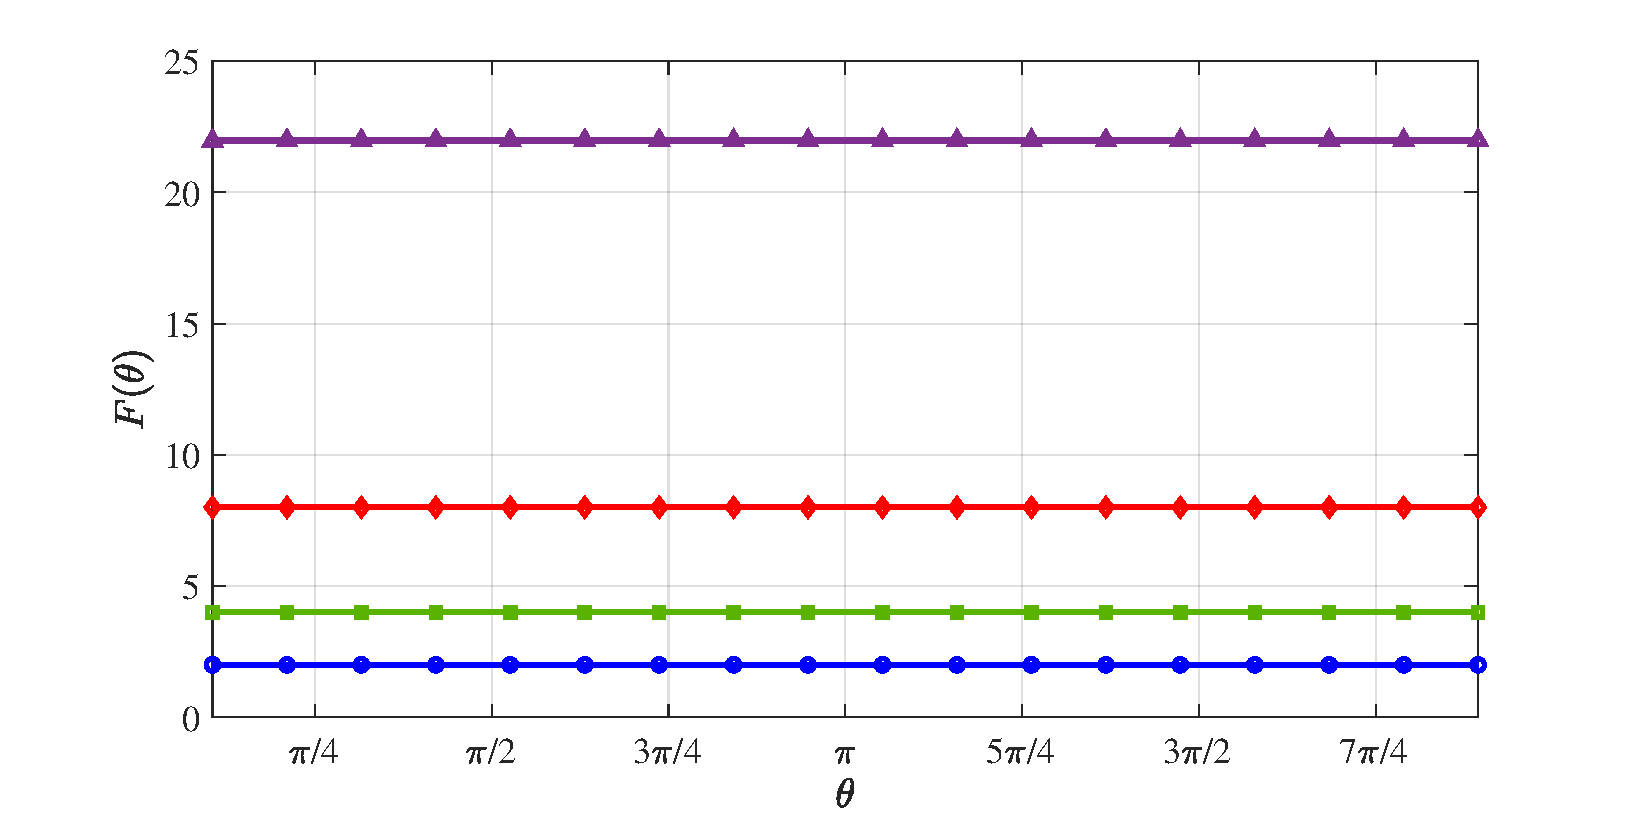
\includegraphics[trim={1.6cm 0.1cm 1.5cm 0.5cm},clip,width=15.5cm]{pictures/ch4_fig1}
	\caption[Saturation of the Braunstein-Caves inequality for optical schemes]{Quantum Fisher information (solid lines) and its classical counterpart (symbols) for coherent (circles), NOON (squares), twin squeezed vacuum (diamonds) and squeezed entangled (triangles) states, with $\bar{n} = 2$ and a photon counting measurement that has been implemented after the action of a $50$:$50$ beam splitter $U_{\mathrm{BS}} = \mathrm{exp}(-i\frac{\pi}{2}J_x)$. This numerical calculation illustrates the saturation of the Braunstein-Caves inequality for path-symmetric states in equation (\ref{bcavesine}).}
\label{braunsteincaves}
\end{figure}

A common property of these configurations is that they belong to the family of path-symmetric states that we reviewed in section \ref{subsec:optint}, so that each mode is associated with the same mean number of photons and the same photon number variance. For this class of probes Hofmann showed that \cite{HofmannHolger2009}
\begin{align}
F(\theta) &= \int \frac{dm}{p(m|\theta)}\left[\frac{\partial p(m|\theta)}{\partial \theta}\right]^2 = \mathrm{Tr}\left[\rho(\theta) L(\theta) \right]
\nonumber \\
&= 4 \left(\langle \psi_0 |J_z^2| \psi_0\rangle - \langle \psi_0 |J_z| \psi_0\rangle^2 \right) = F_q
\label{bcavesine}
\end{align}
if we implement a photon-counting measurement after the action of a 50:50 beam splitter, the POM elements of this scheme being
\begin{equation}
\left\lbrace \mathrm{exp}\left(-i\frac{\pi}{2}J_x \right) \ketbra{k}\mathrm{exp}\left(i\frac{\pi}{2}J_x\right) \right\rbrace_k,
\label{photonpom}
\end{equation}
with $N_1\otimes N_2 = \int dk~k\ketbra{k}$. That is, the classical Fisher information for path-symmetric probes reaches the bound imposed by the Braunstein-Caves inequality \cite{BraunsteinCaves1994}. In figure \ref{braunsteincaves} we show an explicit calculation illustrating this fact for $\bar{n} = 2$. 

Crucially, this implies that any discrepancy between the mean square error $\bar{\epsilon}_{\mathrm{mse}}$ in equation (\ref{erropt}) and the Cram\'{e}r-Rao bound $\bar{\epsilon}_{\mathrm{cr}} = 1/(\mu F_q)$ must necessarily come from the asymptotic approximation that we discussed in section \ref{theory}.  

\subsection{Prior information analysis}
\label{subsec:prioranalysis}

The first step to apply our numerical strategy is to identify the intrinsic width $W_{\mathrm{int}}$ of each state for a given $\bar{n}$ and the POM in equation (\ref{photonpom}), recalling that we have defined $W_{\mathrm{int}}$ as the largest value that the intrinsic width $W_0$ can take such that the likelihood $p(\boldsymbol{m}|\boldsymbol{\theta})$ is concentrated around a single absolute maximum. Some of the random simulations that are required to achieve this goal are shown in figure \ref{priornonasymtptotic}, which allow us to deduce the size of the maximum width by direct examination. The algorithm employed to generate them can be found in appendix \ref{sec:priormatlab}.

For a twin squeezed vacuum and a squeezed entangled state we have found that $W_{\mathrm{int}} = \pi/2$, while coherent states have $W_{\mathrm{int}} = \pi$. Note that those results hold for any $\bar{n}$. On the contrary, with NOON states we have that $W_{\mathrm{int}} = \pi/\bar{n}$ or $W_{\mathrm{int}} = \pi/(2\bar{n})$ depending on whether the value for $N = \bar{n}$ in equation (\ref{noon}) is even or odd, provided that we choose a prior centred around $\bar{\theta} = W_{\mathrm{int}}/2$. 

\begin{figure}[t]
\centering
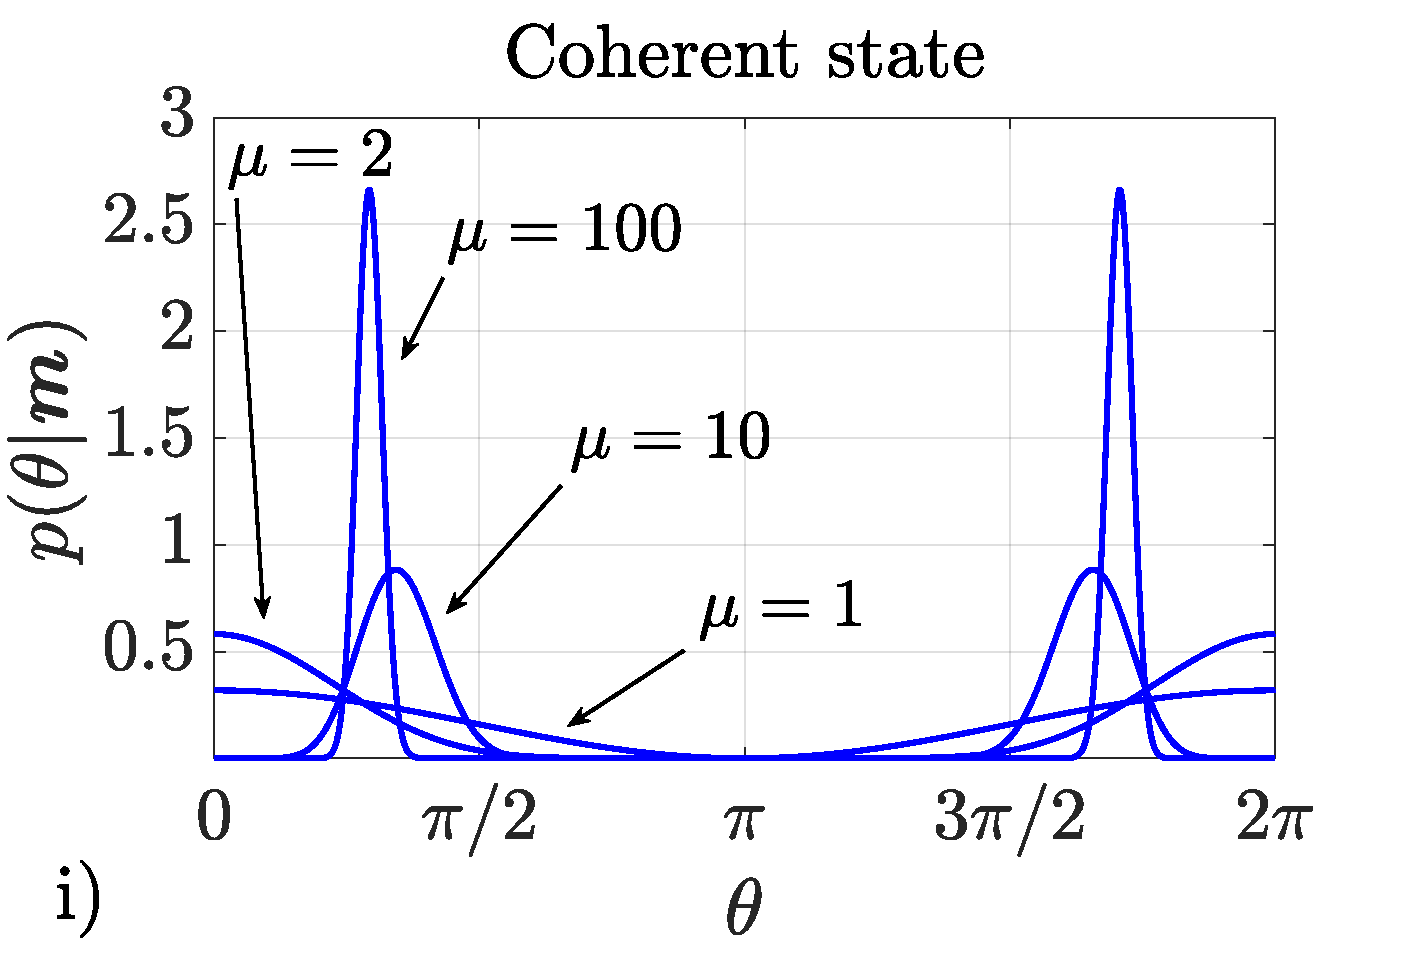
\includegraphics[trim={0cm 0.1cm 0cm 0cm},clip,width=7.85cm]{pictures/ch4_fig2i}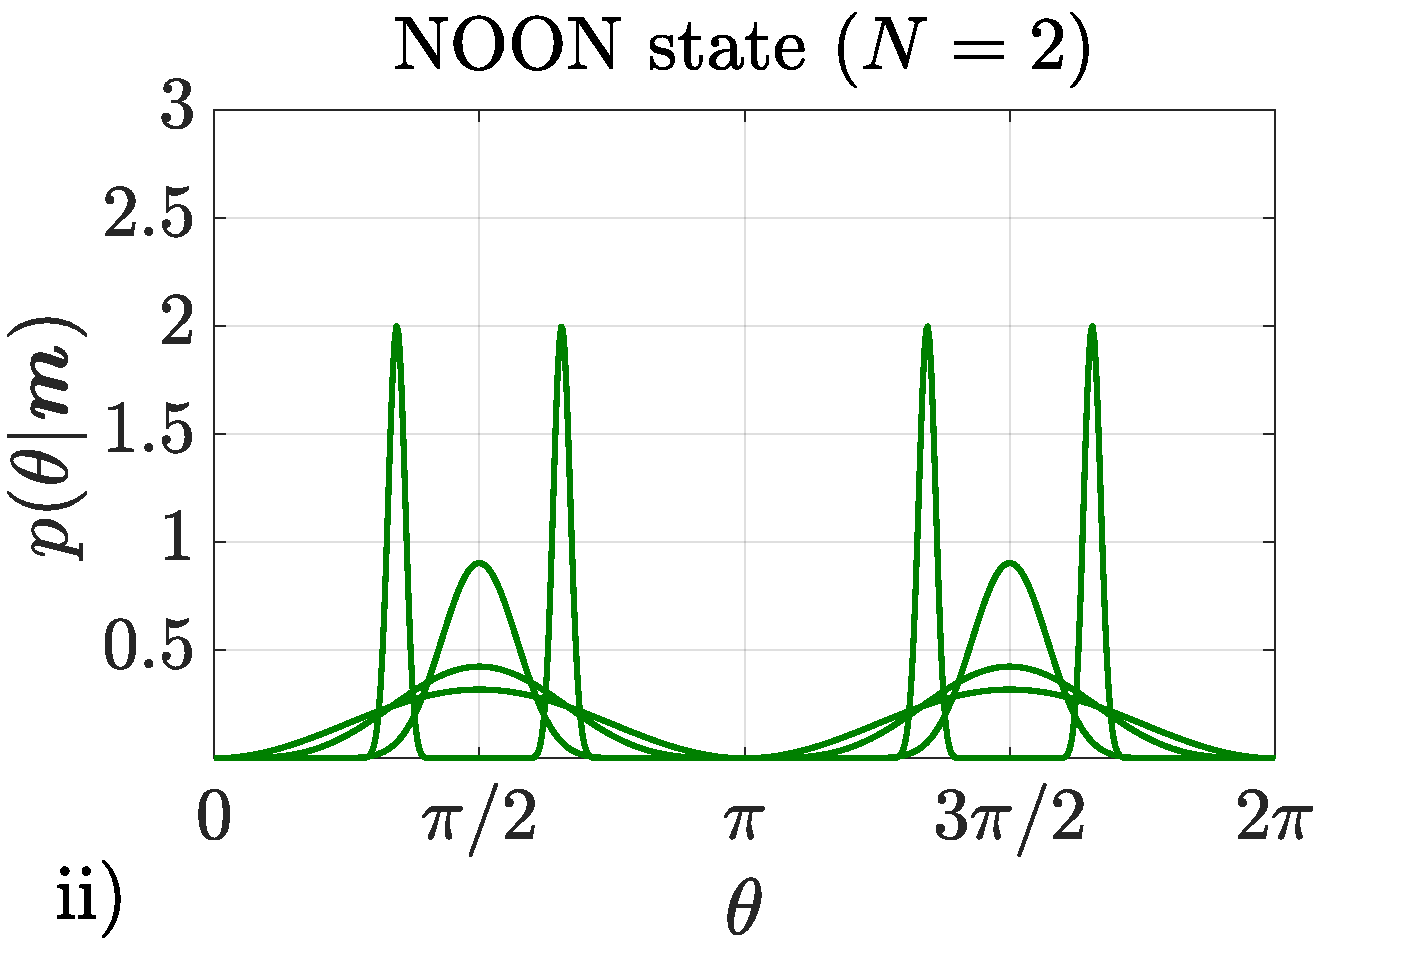
\includegraphics[trim={0cm 0.1cm 0cm 0cm},clip,width=7.85cm]{pictures/ch4_fig2ii}
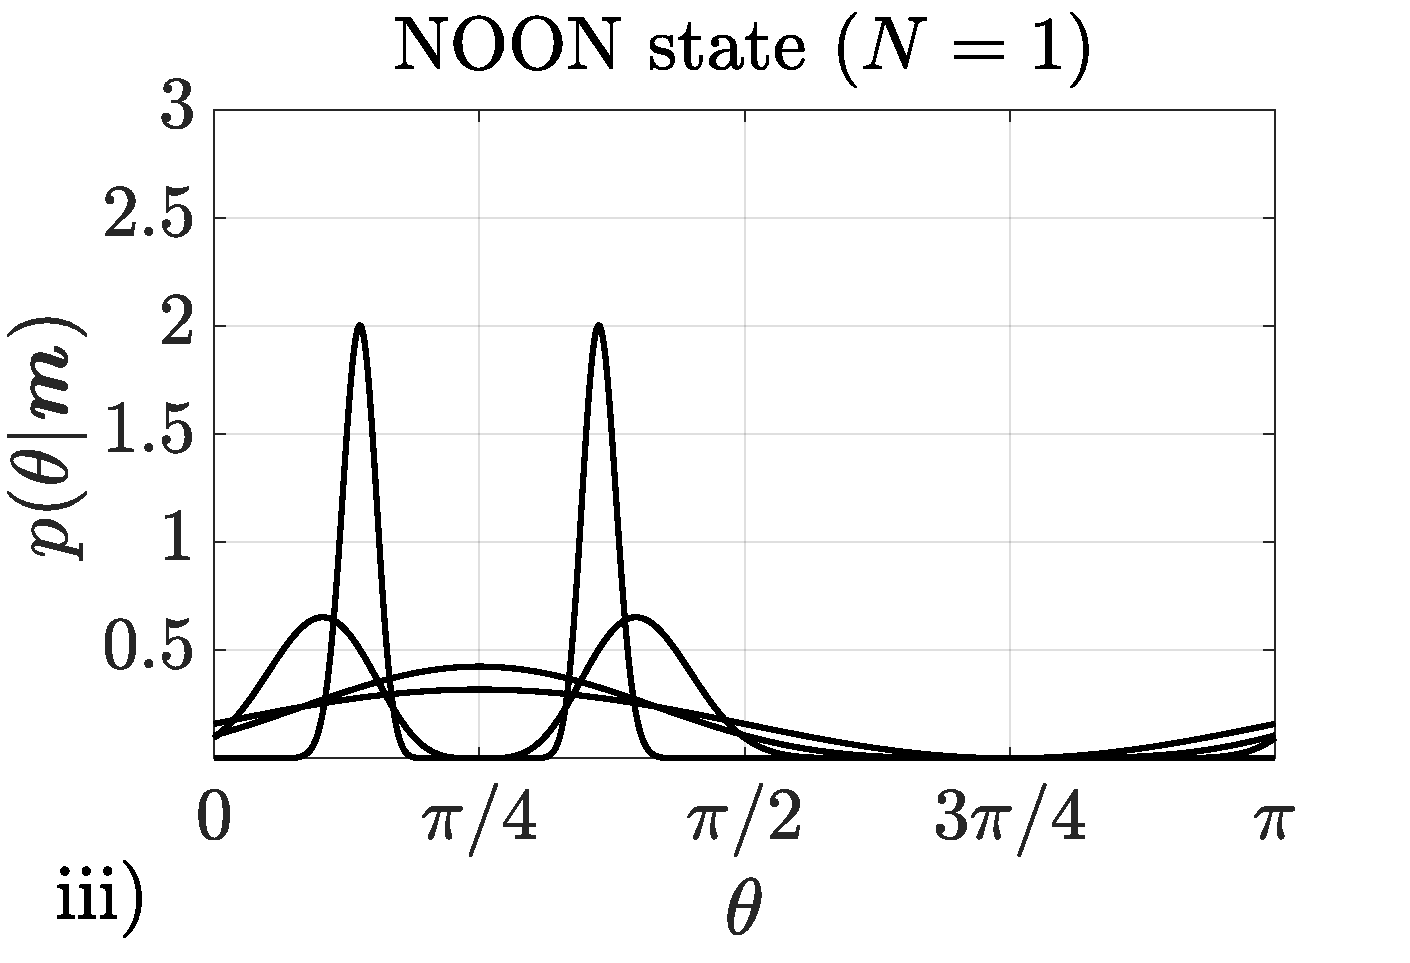
\includegraphics[trim={0cm 0.1cm 0cm 0cm},clip,width=7.85cm]{pictures/ch4_fig2iii}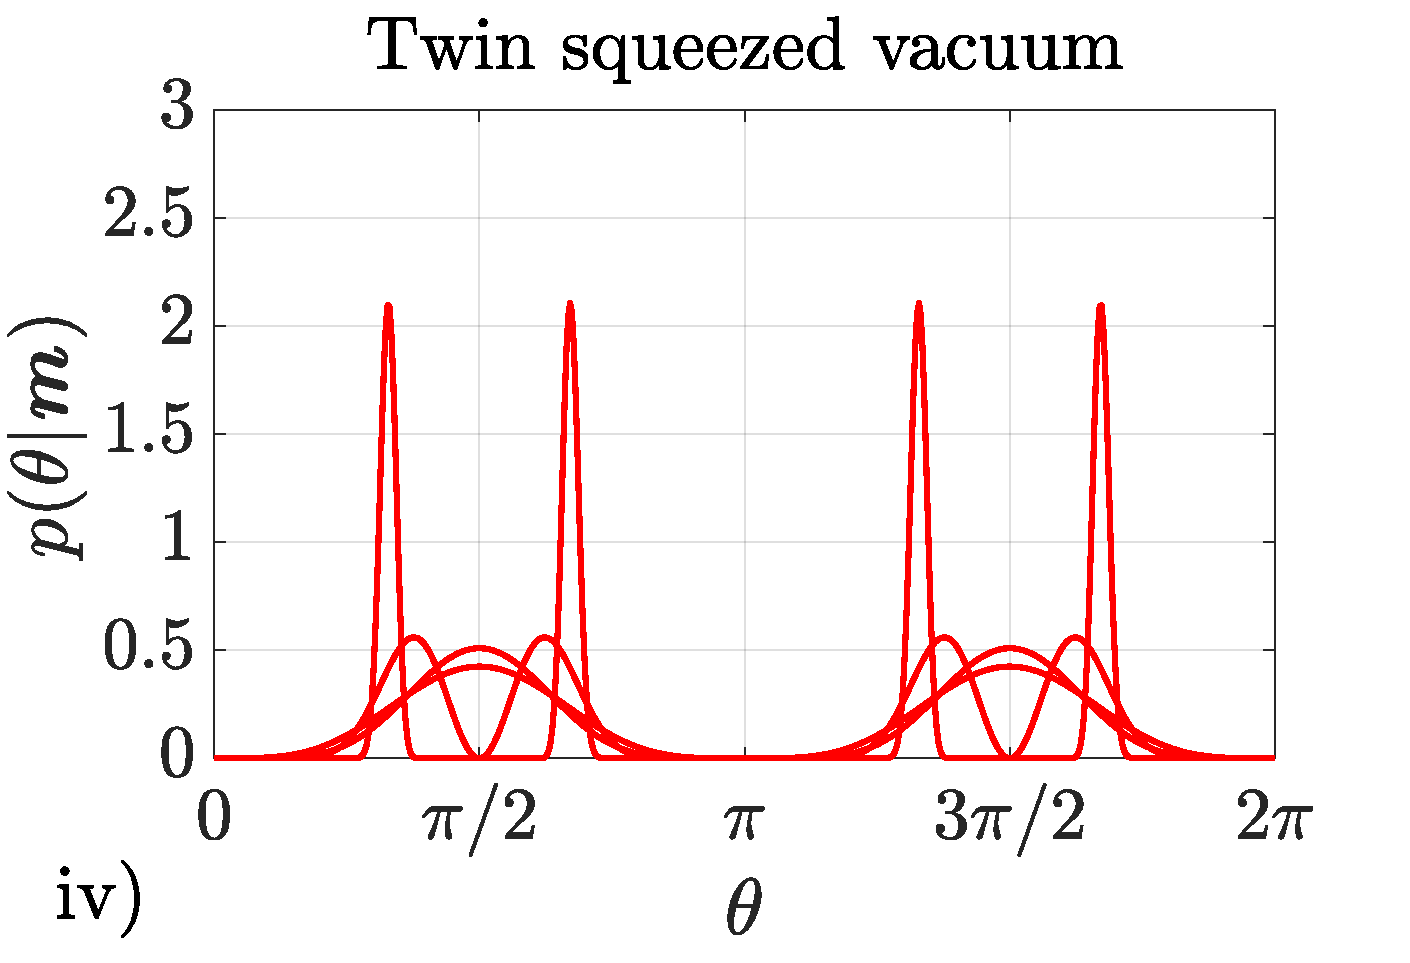
\includegraphics[trim={0cm 0.1cm 0cm 0cm},clip,width=7.85cm]{pictures/ch4_fig2iv}
	\caption[Prior information analysis of a single-parameter scheme]{Posterior density functions for random simulations of 1, 2, 10 and 100 trials, a flat prior and a photon-counting measurement implemented after the action of a 50:50 beam splitter. The initial probes are (i) coherent state with $\bar{n} = 2$, (ii) NOON state with $\bar{n} = 2$, (iii) NOON state with $\bar{n} = 1$, and (iv) twin squeezed vacuum with $\bar{n} = 2$. We draw attention to the fact that these configurations cannot distinguish a unique value  when the initial prior is set to $W_0 = 2\pi$, even if we are in the asymptotic regime with $\mu \gg 1$.}
\label{priornonasymtptotic}
\end{figure}

The value of $W_{\mathrm{int}}$ for coherent states was also determined in \cite{kolodynski2014} by examining the regions where the single-shot likelihood function $p(m|\theta)$ increases or decreases monotonically as a function of $\theta$. This motivates the search of an alternative way of determining $W_{\mathrm{int}}$ by studying the form of $p(m|\theta)$.

From figure (\ref{priornonasymtptotic}) we observe that the posterior $p(\theta|m) \propto p(m|\theta)$ of our schemes presents two types of symmetry: the periodicity of an imaginary envelope and an axis of symmetry within each period. We can formalise these by imposing
\begin{align}
p(m|\theta) &= p(m|\theta + \mathcal{T}),
\nonumber \\
p(m|\mathcal{S} - \theta) &= p(m|\mathcal{S} + \theta)
\label{symconstr}
\end{align}
when the prior is flat, where $\mathcal{T}$ is the period of the envelope and $\mathcal{S}$ is the position of the axis of symmetry. In addition, a form of the second condition that is more useful in calculations is
\begin{equation}
p(m|\theta) = p(m|2\mathcal{S}-\theta),
\label{easiersym}
\end{equation}
which is found after introducing the change of variables $\theta \rightarrow \mathcal{S} - \theta$.

Let us check whether the previous idea allows us to recover the intrinsic width that our numerical method associates with NOON states. The single-shot likelihood function of this scheme is
\begin{equation}
p(n_1, n_2 | \theta) = || \langle n_1, n_2 | \mathrm{e}^{-i\frac{\pi}{2}J_x} \mathrm{e}^{-i J_z \theta}| \psi_0 \rangle ||^2,
\end{equation}
where $\ket{\psi_0}$ is the NOON state in equation (\ref{noon}) and we have changed the notation as $m \rightarrow (n_1,n_2)$ to make the fact that each port has its own output explicit. A lengthy but straightforward calculation that we include in appendix \ref{sec:optrans} shows that
\begin{equation}
p(n_1, n_2 | \theta) = p(n,N-n|\theta) = \frac{2 N! \hspace{0.2em} \mathrm{cos}^2\left[N\theta/2 + (2n-N)\pi/4\right]}{2^N n! (N-n)!}.
\end{equation}
Introducing this probability in the periodicity condition of equation (\ref{symconstr}), and recalling that $\mathrm{cos}^2(x)=[1+\mathrm{cos}(2x)]/2$, we have that 
\begin{eqnarray}
\mathrm{cos}\left(x_{n,N}\right) = \mathrm{cos}\left(x_{n,N} + N\mathcal{T}\right) = \mathrm{cos}\left(x_{n,N}\right)\mathrm{cos}\left(N \mathcal{T} \right)  - \mathrm{sin}\left(x_{n,N}\right)\mathrm{sin}\left(N \mathcal{T} \right),
\end{eqnarray}
with $x_{n,N} = N\theta + (2n-N)\pi/2$, and this implies that
\begin{equation}
\mathcal{T} = \frac{2\pi k}{N}, ~~ \text{with}~~k=0, \pm 1, \pm 2, \dots.
\label{periodicity}
\end{equation}
Similarly, from the condition in equation (\ref{easiersym}) we find
\begin{align}
\mathrm{cos}\left(x_{n,N}\right) = &~\mathrm{cos}\left[2\mathcal{S}N + \left(2n - N\right)\pi - x_{n, N}\right]
\nonumber \\
= &~\mathrm{cos}\left(x_{n,N}\right)\mathrm{cos}\left[2\mathcal{S}N + \left(2n - N\right)\pi \right]  
\nonumber \\
& + \mathrm{sin}\left(x_{n,N}\right)\mathrm{sin}\left[2\mathcal{S}N + \left(2n - N\right)\pi \right],
\end{align}
so that
\begin{equation}
\mathcal{S} = \frac{\pi\left(k-n\right)}{N} + \frac{\pi}{2},  ~~ \text{with}~~k=0, \pm 1, \pm 2, \dots.
\label{mirrorsymmetry}
\end{equation}

To guarantee that the products of single-shot likelihoods do not generate symmetric absolute maxima we need an interval where the likelihood of a single trial does not contain redundant information. Equation (\ref{periodicity}) means that the width of such interval must be  equal to or less than the period $2\pi/N$. In addition, given that
\begin{equation}
\mathcal{S}(k+1) - \mathcal{S}(k) = \frac{\pi}{N}
\end{equation}
for the points of symmetry in equation (\ref{mirrorsymmetry}), we see that, actually, the width cannot be larger than $\pi/N$. We also notice that the axes of symmetry in equation (\ref{mirrorsymmetry}) only contain the point $\theta = 0$ when $2(n-k) = N$, which can only happen when $N$ is even. If $N$ is odd, then we may find $\theta = 0$ as the middle point between axes, since
\begin{equation}
\mathcal{S} \pm \frac{\pi}{2N} = \frac{\pi\left[2\left(k-n\right) \pm 1 \right]}{2N} + \frac{\pi}{2} = 0 ~~\Rightarrow~~ N \pm 1 =2(n-k),
\end{equation}
and the latter condition can be satisfied for odd $N$. As a consequence, if the parameter domain is $[0, W_\mathrm{int}]$, as it is the case in this chapter, then we conclude that $W_\mathrm{int} = \pi/N = \pi/\bar{n}$ when $\bar{n}$ is even, and $W_\mathrm{int} = \pi/(2N) = \pi/(2\bar{n})$ when $\bar{n}$ is odd, since in the latter case only half of the width free of redundancies is included in the domain. We thus arrive in this way at the same result found in the simulations.

This demonstrates that if the analytical formula for the likelihood function is known, then it is sometimes possible to derive the intrinsic width explicitly by analysing the symmetries of the quantum probability for a single shot. Thus our method complements the previous proposal in \cite{kolodynski2014} based on studying the monotonicity of the likelihood. Moreover, our numerical approach provides the means to find $W_\mathrm{int}$ even if the analytical expression for $p(m|\theta)$ is not available, which is sometimes the situation for more complicated states. This is usually the case, for example, when the quantum circuit is designed using state engineering algorithms \cite{knott2016}.

\begin{figure}[t]
\centering
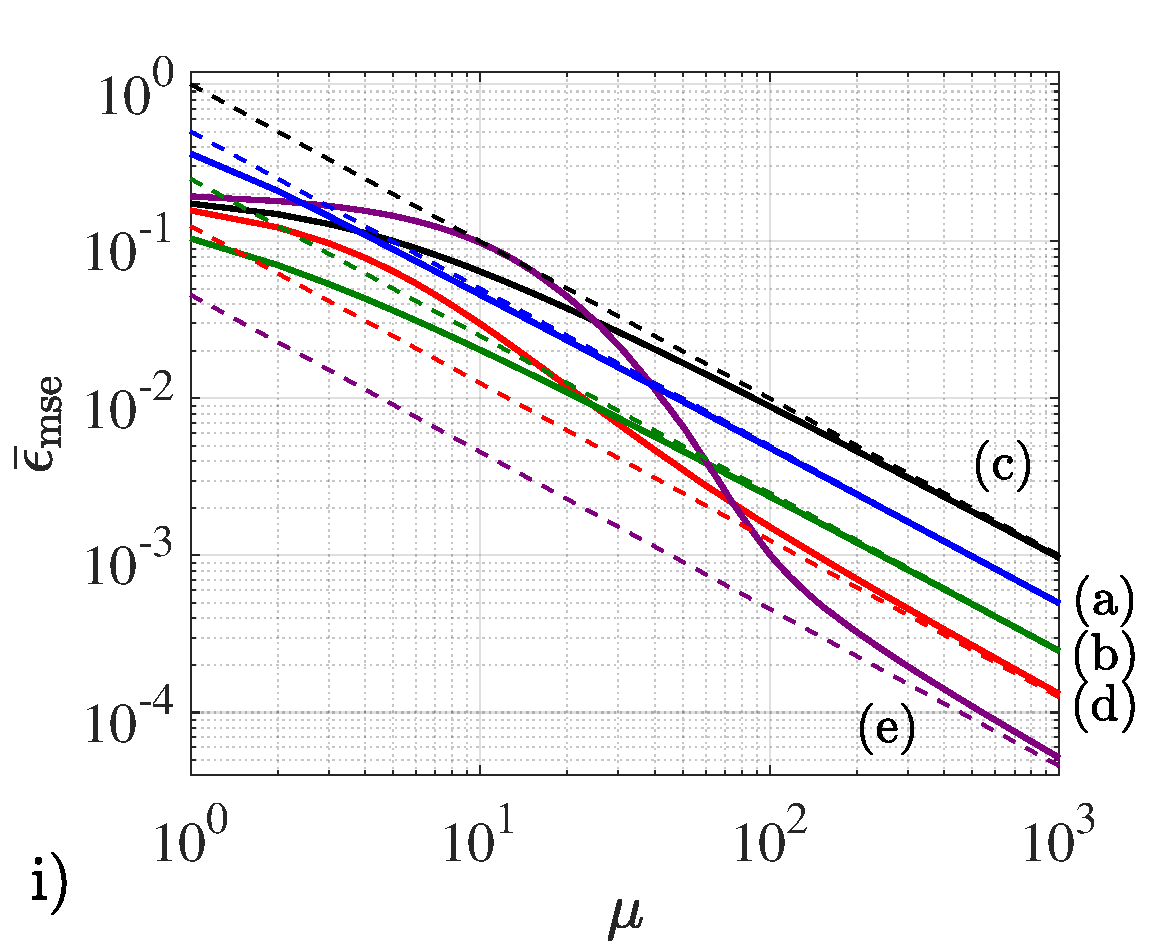
\includegraphics[trim={0.1cm 0.1cm 0.5cm 0.5cm},clip,width=7.7cm]{pictures/ch4_fig3i}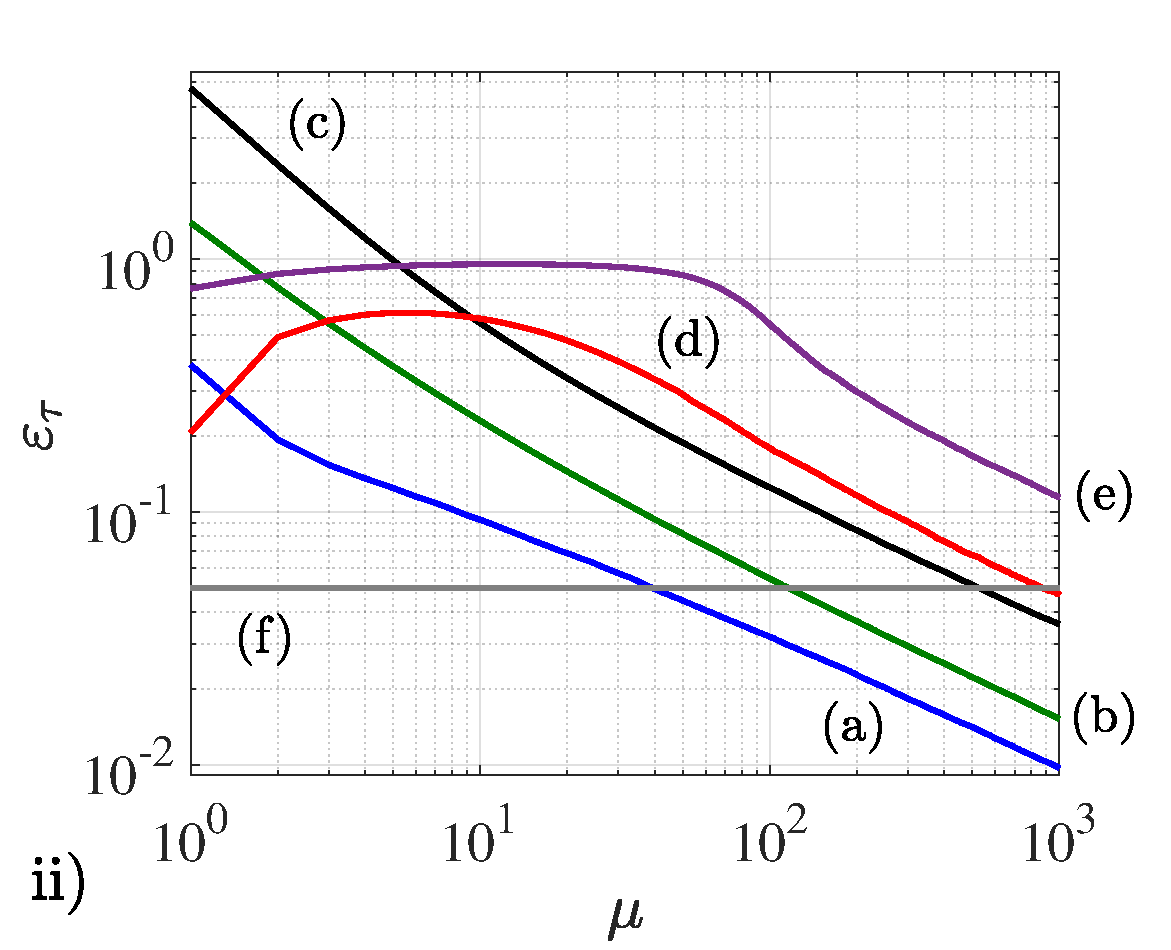
\includegraphics[trim={0.1cm 0.1cm 0.5cm 0.5cm},clip,width=7.7cm]{pictures/ch4_fig3ii} 
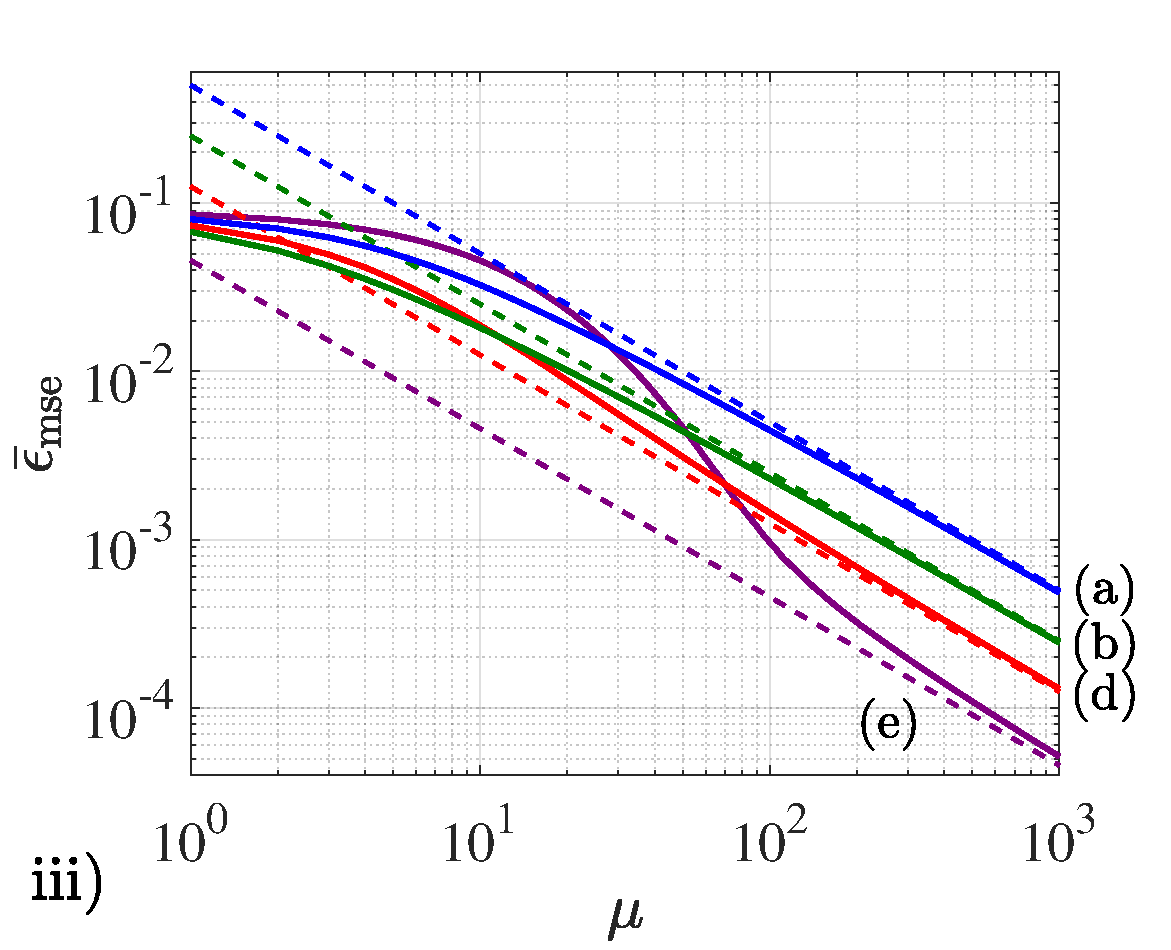
\includegraphics[trim={0.1cm 0.1cm 0.5cm 0.5cm},clip,width=7.7cm]{pictures/ch4_fig3iii}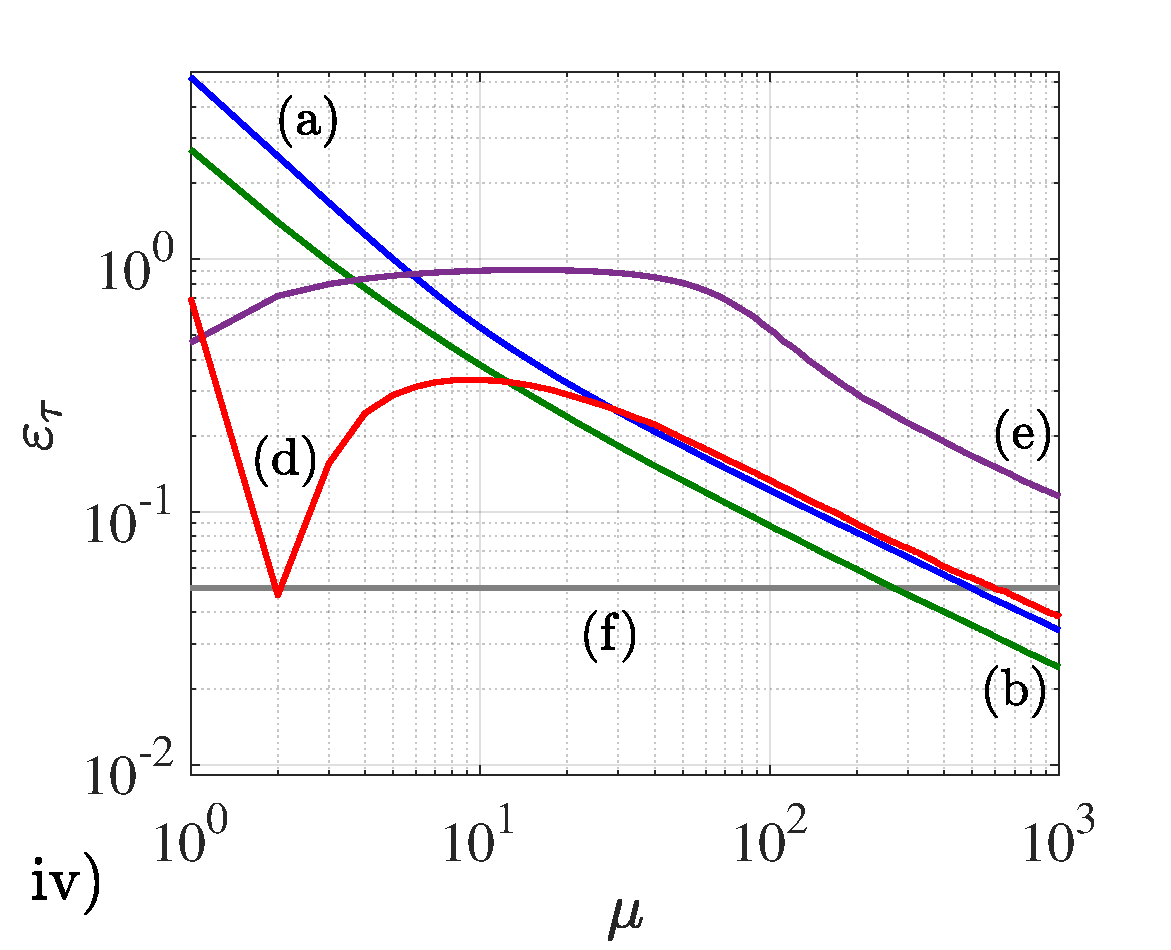
\includegraphics[trim={0.1cm 0.1cm 0.5cm 0.5cm},clip,width=7.7cm]{pictures/ch4_fig3iv}
\caption[Non-asymptotic analysis of the Mach-Zehnder interferometer]{i) Mean square error (solid lines) for the POM in equation (\ref{photonpom}) and quantum Cram\'{e}r-Rao bound (dashed lines) for (a) a coherent state with $\bar{n} = 2$ and $W_{\mathrm{int}} = \pi$, (b) a NOON state with $\bar{n} = 2$ and $W_{\mathrm{int}} = \pi/2$, (c) a NOON state with $\bar{n} = 1$ and $W_{\mathrm{int}} = \pi/2$, (d) a twin squeezed vacuum with $\bar{n} = 2$ and $W_{\mathrm{int}} = \pi/2$, and (e) a squeezed entangled state with $\bar{n} = 2$ and $W_{\mathrm{int}} = \pi/2$, where $\bar{n}$ is the mean number of quanta per trial and $W_{\mathrm{int}}$ is the intrinsic width; (ii) relative error defined by equation (\ref{saturation}) with (f) a threshold $\varepsilon_\tau = 0.05$ for the states considered in figure \ref{mainresult}.i; (iii) repetition of the calculation performed in figure \ref{mainresult}.i with a common prior width $W_0 = \pi/3$ and the same values for $\bar{n}$; and (iv) relative error for the states considered in figure \ref{mainresult}.iii. These results are examined in the main text.}
\label{mainresult}
\end{figure}

The important observation is that none of these states allows us to uniquely identify the relative phase shift when we have no information about its possible values, that is, if $W_0= 2\pi$. We conclude then that the scheme that we are employing introduces some limitations to the estimation protocol, in spite of the fact that the measurement is optimal according to the quantum Cram\'{e}r-Rao bound criterion. 

\subsection{Uncertainty as a function of the number of trials}
\label{subsec:uncertaintynonasymptotic}

Once $W_{\mathrm{int}}$ is known we can use the uniform prior in equation (\ref{prior_probability}) with $W_0 = W_{\mathrm{int}}$ and $\bar{\theta} = W_{\mathrm{int}}/2$ to perform the numerical calculation of the mean square error $\bar{\epsilon}_{\mathrm{mse}}$ in equation (\ref{erropt}), which can be achieved by means of the algorithm described in section \ref{subsec:numalgorithm} (see also appendix \ref{sec:msematlab}). In addition, the algorithm in appendix \ref{subsec:qcrbmatlab} gives the quantum Cram\'{e}r-Rao bound $\bar{\epsilon}_{\mathrm{cr}} = 1/(\mu F_q)$, and the combination of $\bar{\epsilon}_{\mathrm{mse}}$ and $\bar{\epsilon}_{\mathrm{cr}}$ allows us to obtain the relative error $\varepsilon_{\tau}$ in equation (\ref{saturation}). While the explicit form of the optimal estimator $g(\boldsymbol{m}) = \int d\theta p(\theta|\boldsymbol{m})\theta$ will not be provided, note that this is already included within the numerical calculation of $\bar{\epsilon}_{\mathrm{mse}}$.

The results of these operations are shown in figure \ref{mainresult}.i and figure \ref{mainresult}.ii, where we have assumed that the experiment can only be repeated $\mu = 10^3$ times as an extra constraint. For this number of observations, the mean square error of coherent, NOON and twin squeezed vacuum states is close enough to the result predicted by the quantum Cram\'{e}r-Rao bound. In particular, their relative error is smaller than the selected threshold $\varepsilon_\tau = 0.05$. However, the minimum number of observations that are needed in order to reach that threshold is different for different states, and the squeezed entangled state does not even reach it in the regime that we are studying. This state-dependent phenomenon, whose concrete values are indicated in table \ref{table_summary}, has important consequences. 

If we consider first the comparison between a NOON state and a twin squeezed vacuum with $\bar{n} = 2$, $W_{\mathrm{int}} = \pi/2$, we can see that the latter is a better choice according to the Fisher information, but its error is higher for $\mu < 20$. Even if we focus on the results of the asymptotic regime, the twin squeezed vacuum requires $\mu \sim 10^3$ observations to achieve it, while the NOON state only needs $\mu \sim 10^2$. Thus a state whose Fisher information is maximum with respect to other probes can still produce a larger error if the experiment is operating outside of the asymptotic regime. Moreover, although it was shown that only the intra-mode correlations are crucial to surpass the standard quantum limit in the regime where the Fisher approach is valid \cite{sahota2015, sahota2016, proctor2017networked}, this comparison between a NOON state, which includes both types of correlations, and a twin squeezed vacuum, that has intra-mode correlations only, suggests that the role of photon correlations in metrology should be revisited for the non-asymptotic regime. This study will be carried out in detail in section \ref{correlations_section} using a more sophisticated approach.

On the other hand, a coherent state with $\bar{n} = 2$, $W_{\mathrm{int}} = \pi$ is less precise than a NOON state with $\bar{n} = 1$, $W_{\mathrm{int}} = \pi/2$ when $\mu \sim 1$. This implies that there is a region in which a probe with fewer resources can still beat a scheme with more photons if the prior knowledge of the former is higher. By combining these observations with those extracted from the previous probes we conclude that the Cram\'{e}r-Rao bound can both overestimate and underestimate the precision outside of its regime of validity. It is particularly relevant to draw attention to the latter case, since the fact that NOON and coherent states display a mean square error which is lower than their respective Cram\'{e}r-Rao bounds for low values of $\mu$ demonstrates that the unbiased estimators of the local theory are not always optimal.

The analysis of the squeezed entangled state provides further details of the properties of the non-asymptotic regime. In particular, its performance is worse than all the previous cases for $\mu \sim 10$, and it only becomes the best choice when the number of repetitions is greater than $\mu \sim 10^2$. Surprisingly, this result is showing that while states with an indefinite number of photons can do better than the optimal choice for a finite number of quanta, NOON states have the best absolute precision among the cases that we have studied if the number of observations is less than $\mu \sim 10$.

\begin{table} [t]
\centering
{\renewcommand{\arraystretch}{1.05}
\begin{tabular}{|l|c|c|c|c|}
\hline
Probe state & $\bar{n}$ & $W_{\mathrm{int}}$ & $\mu_{\tau} (W_{\mathrm{int}})$ & $\mu_{\tau} (W_0=\pi/3)$\\
\hline
\hline
$|\alpha/\sqrt{2},-i\alpha/\sqrt{2}\rangle$ & $2$ & $\pi$ & $3.9\cdot 10$ & $4.97\cdot 10^2$\\
NOON state (even $N$) & $2$ & $\pi/2$ & $1.15\cdot 10^2$ &$2.67\cdot 10^2$\\
NOON state (odd $N$)& $1$ & $\pi/2$ & $5.26\cdot 10^2$ & - \\
$S_1(r)S_2(r)\ket{0,0}$ & $2$ & $\pi/2$ & $8.74\cdot 10^2$ & $5.95\cdot 10^2$\\
$\mathcal{N}(\ket{r,0}+\ket{0,r})$ & $2$ & $\pi/2$ & $>10^3$ &$ >10^3$\\
\hline
\end{tabular}}
\caption[Conditions to reach the asymptotic regime]{Numerical values of $W_{\mathrm{int}}$ and $\mu_{\tau}$ obtained in figure \ref{priornonasymtptotic} and figure \ref{mainresult}, respectively, for an asymptotically optimal strategy and a threshold $\varepsilon_\tau = 0.05$. The representation of the posterior probability $p(\theta|\boldsymbol{m})$ for the squeezed entangled state that provides the value of its intrinsic width was very similar to that of the twin squeezed vacuum, and therefore it has been omitted in figure \ref{priornonasymtptotic} for brevity. In addition, note that we have chosen $\bar{n} = 2$ for most of our schemes in order to detect a significant improvement over the standard quantum limit.}
\label{table_summary}
\end{table}

To have a fairer comparison, we have repeated the calculation with a common width $W_0 = \pi/3$ and $\bar{n} = 2$. Figures \ref{mainresult}.iii and \ref{mainresult}.iv show that, while the numerical values are different, the qualitative conclusions are the same. Nonetheless, there is an important difference given that the prior knowledge is now higher. For the NOON and coherent states, $\mu_{\tau}$ has increased with respect to the previous calculation, since the starting difference between the error and the bound is now greater. On the other hand, for the twin squeezed vacuum there is a point where now the mean square error crosses the Cram\'{e}r-Rao bound before a stable saturation is reached. This happens because for $W_0 = W_{\mathrm{int}}$ the error approached the bound from above, while for $W_0 = \pi/3$ the error begins below the bound and then crosses it to achieve the asymptotic regime from above. This suggests that if we keep increasing our prior information and we make the width of the parameter domain very small, then the number of observations needed to approach the Cram\'{e}r-Rao bound will grow. 

\subsection{A practical relation to prevent \emph{infinite-precision} states}
\label{subsec:infiniteprecision}

It is possible to formalise the previous phenomenon and derive an intuitive and informative relation that detects states that are not well-behaved. Firstly, we note that the uncertainty of an estimation that is made before we perform the experiment is represented by the variance of the prior probability 
\begin{equation}
\bar{\epsilon}_{\mathrm{mse}}({\mu = 0}) = \Delta \theta^2_p = \int d\theta p(\theta) \theta^2 - \left[\int d\theta p(\theta) \theta \right]^2
\end{equation}
that we introduced in section \ref{subsec:originalderivation}, which for the flat density in equation (\ref{prior_probability}) is
\begin{equation}
\Delta \theta^2_p = \left(\bar{\theta}^2 + \frac{W_0^2}{12}\right) - \bar{\theta}^2 = \frac{W_0^2}{12}.
\end{equation}
On the other hand, we know that the precision is given by the Fisher information when $\mu \gg 1$; consequently, an estimation protocol is only worthwhile when
\begin{equation}
\Delta \theta^2_p(\rho) > \frac{1}{\mu(\rho) F_q(\rho)}
\label{criterion}
\end{equation}
is asymptotically satisfied, where we have made explicit the dependence on the state to indicate that the values of $\mu$ and $\Delta \theta^2_p$ guarantee that the Cram\'{e}r-Rao regime can be reached. If equation (\ref{criterion}) were not fulfilled, then the experiment would not be telling us more than what we already knew. By reorganizing the terms we  arrive at
\begin{equation}
\mu(\rho) > \frac{1}{\Delta \theta^2_p(\rho) F_q(\rho)},
\label{fundamental}
\end{equation}
which is a constraint based on practical requirements.

According to equation (\ref{fundamental}), the number of required observations will increase when the Fisher information is fixed and the prior knowledge is improved, which is consistent with the results of figure \ref{mainresult}. Furthermore, we have seen that the prior width cannot be arbitrarily large if we want to employ certain states in an experiment. Thus, if we maximise the Fisher information at the expense of decreasing the maximum prior uncertainty, and the latter phenomenon is faster, then the number of observations will tend to infinity\footnote{It is important to note that equation (\ref{fundamental}) only helps to predict cases where $\mu(\rho)$ grows indefinitely. Any other finite result will constitute a necessary but not sufficient condition that the value of the number of observations needed to reach the asymptotic regime must satisfy.}.

This is precisely the case of the family of one-mode states
\begin{equation}
\ket{\psi_0} = \sqrt{1 - \delta}\ket{0} + \sqrt{\delta}\ket{N/\delta}
\label{infinite}
\end{equation}
that was considered, e.g., in \cite{alfredo2017}, where $0 < \delta < 1$ and $N/\delta$ is an integer. To see it, 
first we perform an analysis of the periodicity associated with the unitary transformation 
\begin{equation}
\ket{\psi(\theta)} = \sqrt{1-\delta}\ket{0} + \sqrt{\delta}\mathrm{e}^{-i\theta N/\delta}\ket{N/\delta}. 
\end{equation}
By imposing $\ket{\psi(\theta)} = \ket{\psi(\theta + \mathcal{T})}$ we find that
\begin{equation}
\mathrm{exp}\left(-i N\theta/\delta\right)=\mathrm{exp}\left(-i N\theta/\delta\right)\mathrm{exp}\left(-i N\mathcal{T}/\delta\right),
\end{equation}
which implies that $\mathcal{T} = 2\pi k\delta/N$, with $k = 0, \pm 1, \pm 2, \dots$. This indicates that $W_{\mathrm{int}} \leqslant 2\pi\delta/N$, so that $\Delta \theta^2_p \leqslant \pi^2 \delta^2/(3N^2)$ when $W_0 = W_\mathrm{int}$. Furthermore, the Fisher information is
\begin{eqnarray}
F_q = 4[ \langle \psi_0 | (a^\dagger a )^2 | \psi_0 \rangle - \langle \psi_0 | a^\dagger a  | \psi_0 \rangle^2] = 4\left(\frac{N^2}{\delta} - N^2 \right) = \frac{4N^2(1-\delta)}{\delta}.
\end{eqnarray}
Hence, from equation (\ref{fundamental}) we have that
\begin{equation}
\mu(\delta) > \frac{3}{4\pi^2 \delta (1- \delta)}.
\label{infinitesolution}
\end{equation}
The Fisher information suggests that we can get an infinite precision in the limit $\delta \rightarrow 0$ for a fixed number of resources per trial $\bar{n} = N$, but equation (\ref{infinitesolution}) shows that this conclusion only holds if the total number of resources is actually infinite, which is consistent with the analyses of sub-Heisenberg strategies in the literature \cite{tsang2012, berry2012infinite, hall2012}. From a physical point of view we conclude that it is not advantageous to use states for which the majority of our resources have to be employed in making our scheme as sensitive as the prior uncertainty that we already had.

\section{Summary of results and conclusions}

The first step of our methodology, which combines the optimal Bayes estimator with a quantum strategy that is asymptotically optimal, has been implemented in a numerical fashion. This process has involved a rigorous analysis of the prior knowledge required by given state and POM and the estimation of the number of repetitions that are needed to reach the asymptotic regime. This has allowed us to explore the limitations of approximating the Bayesian mean square error by the quantum Cram\'{e}r-Rao bound for practical scenarios that are relevant in quantum metrology, to characterise the boundary that separates the asymptotic and non-asymptotic regimes, and to perform a first analysis of the non-asymptotic regime. 
 
We have applied this strategy to coherent, NOON, twin squeezed vacuum and squeezed entangled states for the estimation of phase shifts in optical interferometry, finding that the conditions for approaching the Cram\'{e}r-Rao bound crucially vary with the state of the system once the POM has been fixed. Moreover, we have proposed a simple and practical criterion to detect states that may require an infinite amount of trials before they provide useful information beyond the prior knowledge.

From the results of our simulations we can conclude that maximizing the Fisher information alone is not always enough to find the best precision in general. For instance, while a twin squeezed vacuum outperforms NOON states according to the Fisher information, we have found that this conclusion may not hold when the number of observations is low. Similarly, a squeezed entangled state is asymptotically better than the previous examples, but it is the worst choice for small values of $\mu$ among the schemes that we have examined. In fact, a coherent state with no correlations and a NOON state with less photons per observation outperform it when $\mu \sim 10$. An additional lesson extracted from section \ref{results} is that the role of inter-mode and intra-more correlations and the use of states with an indefinite number of quanta to enhance the precision needs to be revisited in the non-asymptotic regime.

As a consequence, for a real experiment either we need to perform a fully Bayesian analysis or we must estimate explicitly the number of observations that are required to guarantee that we are operating in the asymptotic regime if we want to follow the path of the Fisher information. This practice will improve the quality and fairness of the comparisons between strategies, helping us to understand the fundamental limits of estimation theory and aiding the design of quantum sensing protocols for quantum technologies. A clear demonstration of the latter can be found in \cite{jesus2018dec}
\begin{displayquote}
\emph{Designing quantum experiments with a genetic algorithm}, Rosanna Nichols, Lana Mineh, \underline{Jes\'{u}s Rubio}, Jonathan C. F. Matthews and Paul A. Knott, Quantum Sci. Technol. 4 045012 (2019).
\end{displayquote}
where in collaboration with the University of Nottingham and the University of Bristol we succeeded in combining the methods of this chapter with a genetic algorithm in order to design optical experiments that can be accessed with current technology. This proposal will be examined in section \ref{sec:genetic} once we have completed our methodology for single-parameter estimation protocols. 

Finally, we notice that the contents in this chapter have been published in \cite{jesus2017}
\begin{displayquote}
\emph{Non-asymptotic analysis of quantum metrology protocols beyond the Cram\'{e}r-Rao bound}, \underline{Jes\'{u}s Rubio}, Paul Knott and Jacob Dunningham, J. Phys. Commun. 2 015027 (2018).
\end{displayquote}